\chapter{Alberi di decisione}
Gli alberi di decisione sono uno dei metodi più utilizzati nella pratica per l'inferenza induttiva.
L'obiettivo è quello di imparare ad approssimare funzioni su valori discreti, in modo da poter modellare espressioni disgiuntive e al tempo stesso essere robusti rispetto a dati rumorosi.
La funzione appresa viene rappresentata come un albero, in maniera alternativa come usa serie di \texttt{if-then-else}.
Riprendendo i concetti di approssimazione di una funzione:
\begin{itemize}
	\item $X$ è l'insieme delle istanze.
	\item $Y$ è l'insieme delle etichette (classi).
	\item $f: X \rightarrow Y$ è la funzione target (sconosciuta).
	\item $G=\{g: X \rightarrow Y\}$ è l'insieme delle ipotesi.
\end{itemize}
L'input del problema è l'insieme di esempi della funzione target $F$ di addestramento
$\{<x_i, y_i>\}_{i=1}^n$
e l'output è l'ipotesi $h \in G$ che approssima meglio $f$.
Come avviene l'approssimazione negli alberi di decisione?
Ogni $x\in X$ è un'istanza, ovvero un vettore di feature. I valori di $Y$ sono discreti.
Ogni funzione $g$ è un albero, dove $x$ viene classificato scendendo nell'albero fino alle foglie, dove gli viene assegnata una $y$.
\begin{figure}[h]
	\centering
	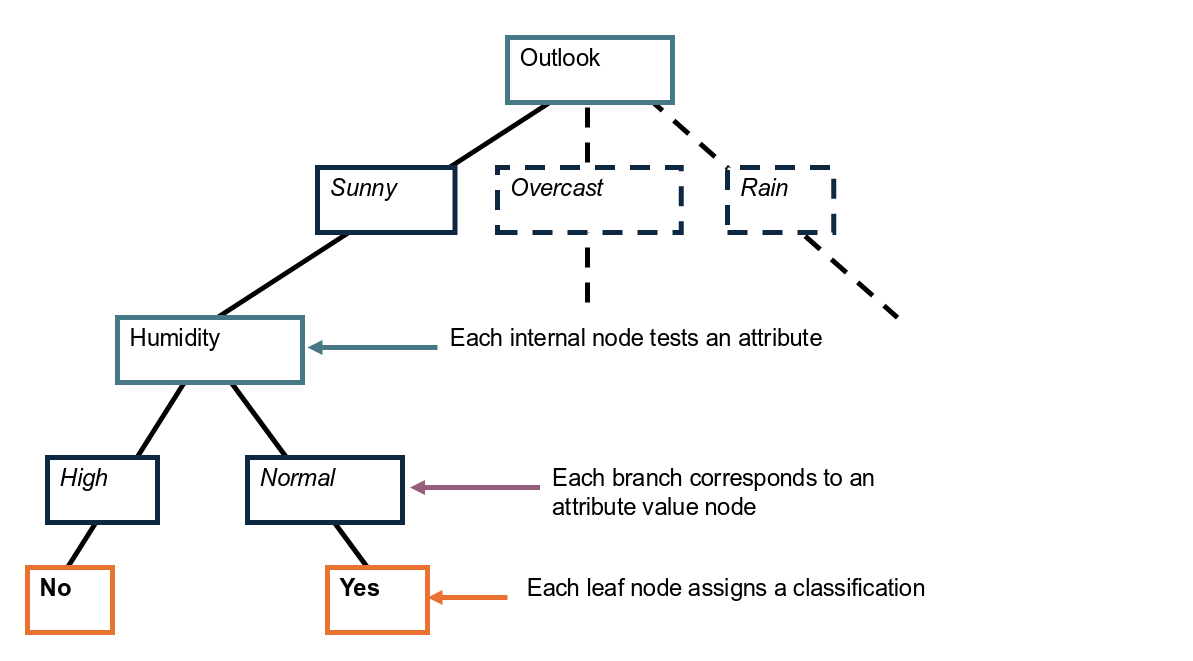
\includegraphics[width=0.8\textwidth]{pictures/decisionTree.png}
	\caption{Esempio di albero di decisione per la classificazione }
\end{figure}
Da notare che non tutti gli attributi necessariamente concorrono alla classificazione.
Gli alberi di decisione rappresentano quindi disgiunzioni di congiunzioni di condizioni sugli attributi.
Questo perché ogni cammino dalla radice a una foglia rappresenta una congiunzione di condizioni sugli attributi, l'insieme dei cammini che portano a una stessa etichetta rappresenta una disgiunzione di congiunzioni.
\\
Perché usare gli alberi di decisione?
Esplicitano la relazione tra attributi e sono facilmente interpretabili.
\\ \\
Consideriamo allora l'insieme di disgiunzioni di congiunzioni, se non ci sono esempi contraddittori allora la formula è vera per ogni esempio positivo e falsa per ogni esempio negativo,
dunque è consistente con il dataset di addestramento.
Vogliamo però inoltre che la formula sia il più piccola possibile (rimanendo valida), dato che è la nostra euristica per una buona generalizzazione.
Vogliamo trovare la formula equivalente minima.
Posso rimuovere controlli non necessari, ad esempio se ho la formula
\[
(\mathrm{Outlook}=\mathrm{Rain}) \land (\mathrm{Temperature}=\mathrm{Hot}) \land (\mathrm{Humidity}=\mathrm{High}) \land (\mathrm{Wind}=\mathrm{Weak}) \lor
\]
\[
(\mathrm{Outlook}=\mathrm{Rain}) \land (\mathrm{Temperature}=\mathrm{Hot}) \land (\mathrm{Humidity}=\mathrm{High}) \land (\mathrm{Wind}=\mathrm{Strong})
\]
dato che l'ultimo attributo non influenza il risultato (weak e strong sono tutti i possibili valori di wind) posso rimuoverlo, ottenendo
\[
(\mathrm{Outlook}=\mathrm{Rain}) \land (\mathrm{Temperature}=\mathrm{Hot}) \land (\mathrm{Humidity}=\mathrm{High}).
\]
Un altro caso è quando due o più congiunzioni contengono la stessa sottoformula, dunque non dovrebbero essere valutate nuovamente.
\\
Gli alberi di decisione dividono lo spazio delle feature in iper rettangoli con assi paralleli agli assi delle feature.
Ogni regione rettangolare viene etichettata con una classe (o una distribuzione di probabilità sulle classi).
\begin{figure}[h]
	\centering
	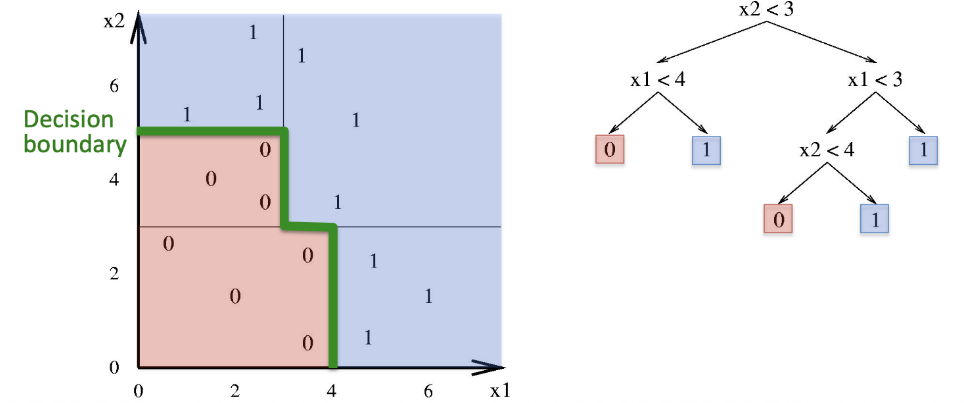
\includegraphics[width=\textwidth]{pictures/decisionBoundary.png}
	\caption{Esempio di partizionamento dello spazio delle feature tramite un albero di decisione}
\end{figure}
Questo partizionamento è chiamato \textit{decision boundary}.
\section{Espressività degli alberi di decisione}
Gli alberi di decisione possono esprimere qualsiasi funzione sugli attributi di un input.
Trivialmente, esiste un albero di decisione consistente per ogni insieme di training con un cammino verso una foglia per ogni esempio, ma probabilmente questo non generalizzerà per nuovi esempi.
Un "buon" attributo separa gli esempi in sottoinsiemi che sono (idealmente) tutti negativi o tutti positivi.
\begin{figure}[H]
	\centering
	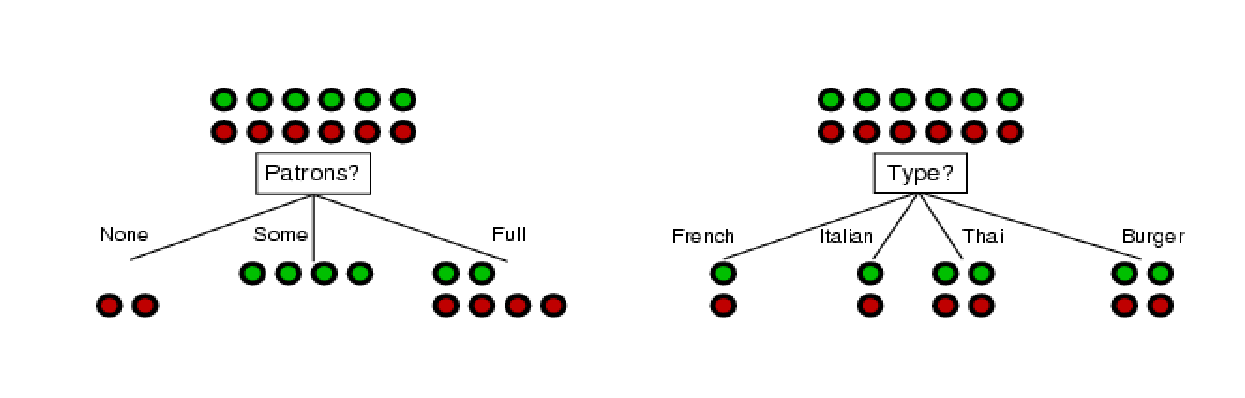
\includegraphics[width=0.8\textwidth]{pictures/separazioneDT.png}
	\caption{Esempio di albero di decisione che rappresenta la funzione XOR}
	\label{fig:DTsep}
\end{figure} \noindent
Osservando la figura \ref{fig:DTsep}, quale attributo separa meglio gli esempi? Patrons, perché divide gli esempi in due insiemi, uno con tutti esempi positivi e uno con esempi negativi e positivi, tranne in un ramo in cui ho una distribuzione.
Nel secondo esempio invece non siamo in grado di separare gli esempi basandoci su quell'attributo.
\\ \\
Al crescere del numero di nodi (o la profondità) dell'albero, cresce la dimensione dello spazio delle ipotesi.
Quanti alberi di decisione distinti ci sono con $n$ attributi booleani?
\begin{itemize}
	\item Il numero di funzioni booleane su $n$ argomenti.
	\item Il numero di tabelle di verità distinte con $2^n$ righe.
	\item $2^{2^n}$ tabelle di verità (dato che ogni riga può essere 0 o 1).
\end{itemize}
\section{Apprendimento degli alberi di decisione}
Gli alberi di decisione effettuano l'analisi del rischio empirico con diverse funzioni di loss in base al problema (regressione o classificazione).
\subsection{Alberi di decisione di classificazione}
Vediamo gli alberi di decisione per la classificazione.
Vogliamo minimizzare il rischio empirico sulla funzione di loss 0-1:
\[
R_{emp}(g) = \frac{1}{n} \sum_{i=1}^n 1(g(x_i) \neq y_i)
\]
Dove la funzione di loss 0-1 è definita come:
\[
L(y, g(x)) = \begin{cases}
0 & \text{se } y = g(x) \\
1 & \text{se } y \neq g(x)
\end{cases}
\]
Qual è un problema con questa funzione di loss?
\begin{figure}[h]
	\centering
	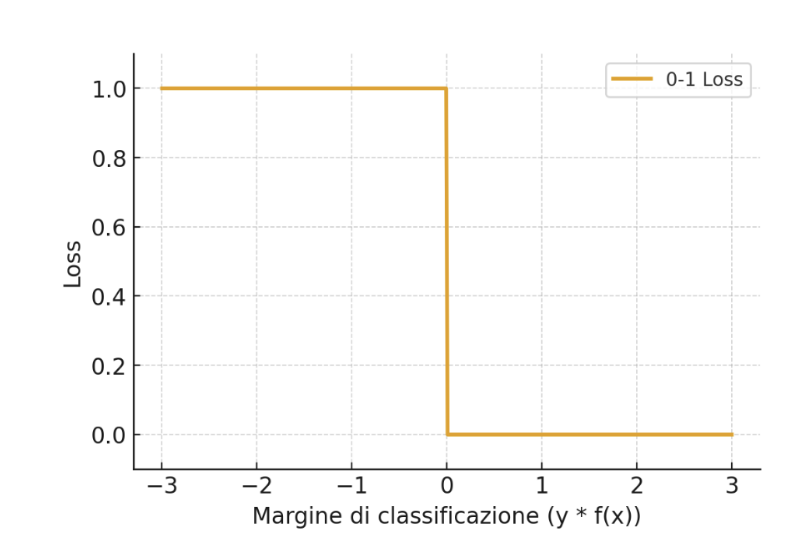
\includegraphics[width=0.7\textwidth]{pictures/loss10.png}
	\caption{Funzione di loss 0-1}
\end{figure}
La funzione di loss 0-1 non è differenziabile, dunque non posso usare metodi basati sul calcolo del gradiente per minimizzarla.
Un modo per aggirare questo problema è usare funzioni di loss surrogate, più facili da computare, che siano differenziabili e che correlino con la funzione di loss originale.
\subsection{Alberi di decisione di regressione}
Come funzione di rischio empirico medio possiamo usare l'errore quadratico medio:
\[
R_{emp}(g) = \frac{1}{n} \sum_{i=1}^n (y_i - g(x_i))^2
\]
\begin{figure}[h]
	\centering
	\includegraphics[width=0.6\textwidth]{pictures/MSE.png}
	\caption{Funzione di loss MSE}
\end{figure}
\subsection{Difficoltà nel training}
In generale fare training di alberi di decisione è un problema NP-completo.
Dunque si usano algoritmi che utilizzano euristiche greedy per costruire l'albero in modo incrementale.
Si inizia da un albero vuoto, e a ogni passo si sceglie il miglior attributo su cui fare lo split, basandosi su una metrica, poi si ripete il processo ricorsivamente.
Inoltre, è possibile fermarsi a un albero parziale, senza arrivare alle foglie, perché?
Secondo il principio del \textbf{rasoio di Occam}, l'ipotesi più semplice che spiega i dati è da preferire.
\begin{figure}[H]
	\centering
	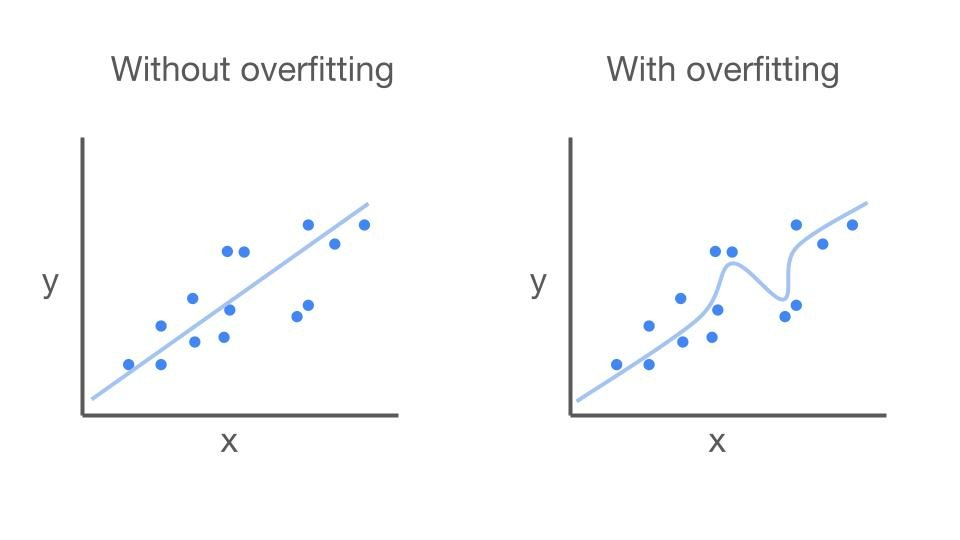
\includegraphics[width=0.8\textwidth]{pictures/overfitting.png}
	\caption{Esempio di overfitting}
\end{figure} 
\begin{figure}[H]
	\centering
	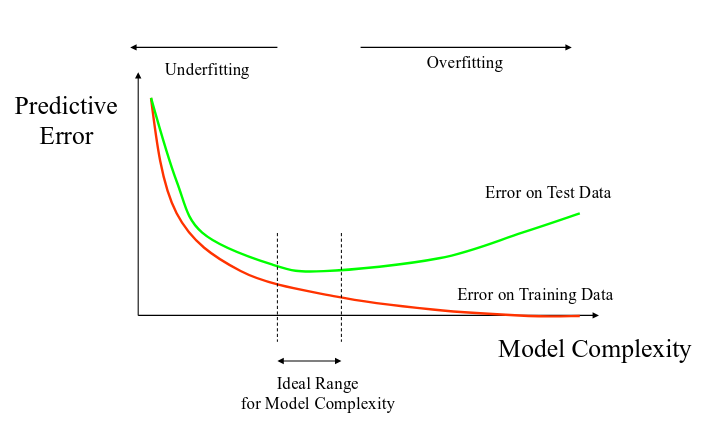
\includegraphics[width=0.8\textwidth]{pictures/overfittingCorrelation.png}
	\caption{Errori in funzione della complessità del modello}
\end{figure}
\begin{figure}[H]
	\centering
	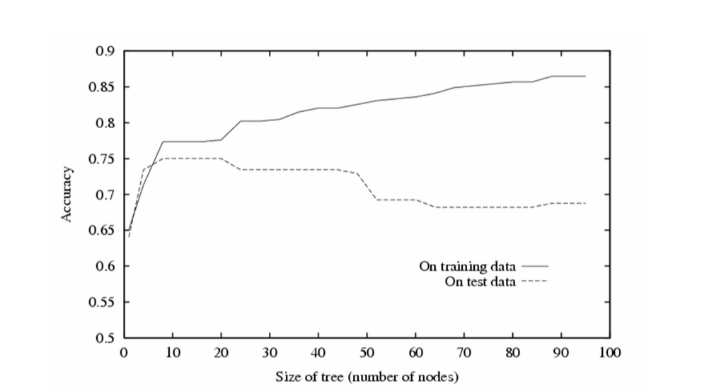
\includegraphics[width=0.8\textwidth]{pictures/overfittingTree.png}
	\caption{Accuratezza in funzione della profondità dell'albero}
\end{figure}
\noindent
Come posso evitare l'overfitting?\\
Posso fermare la crescita dell'albero quando la separazione dei dati non è più significativa, oppure posso creare l'albero intero e poi potare i rami dopo.
\\
Come seleziono il "miglior" albero?
\\
Posso misurare le performance su un training set, oppure usare la usare un dataset di validazione.

\begin{algorithm}[h]
\caption{Algoritmo base per l'apprendimento di alberi di decisione}
\label{alg:decision-tree-basic}
\KwIn{Esempi di addestramento $S$, insieme di attributi $A$}
\KwOut{Albero di decisione con radice \texttt{node}}
\SetKw{KwAnd}{e}
node := radice dell'albero di decisione\;
\While{esistono nodi da espandere}{
  A := scegliere il "miglior" attributo di decisione per il nodo corrente\;
  assegnare A come attributo di decisione per il nodo\;
  \ForEach{valore $v$ di $A$}{
	creare un nuovo discendente del nodo associato a $v$\;
  }
  smistare gli esempi di addestramento ai nodi foglia\;
  \If{gli esempi di addestramento nei nodi foglia sono perfettamente classificati}{
	fermarsi\;
  }
  \Else{
	ricorrere sui nuovi nodi foglia\;
  }
}
\Return{node}\;
\end{algorithm}
